%
% fig/dreieck-konstruktion.tex -- Konstruktion eines gleichseitigen
% Dreiecks aus zwei gegebenen Punkten durch Drehung um 60 Grad.
% Beispielwerte gemaess Praesentation: A=1+i, B=3+i, C=2+(1+sqrt3)i
%
\begin{figure}
\centering
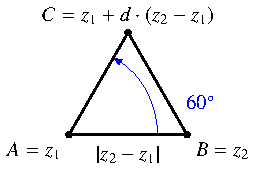
\includegraphics{papers/konstruktion/images/dreieck-konstruktion.pdf}
\caption{Konstruktion des dritten Eckpunkts $C$ eines gleichseitigen
Dreiecks aus zwei gegebenen Punkten $A$ und $B$:
Drehung von $B$ um $A$ um den Winkel $60^\circ$ mit dem Drehfaktor
$d = \cos(60^\circ) + i \sin(60^\circ)$ ergibt $C$.
\label{komplex:figure:dreieck-konstruktion}}
\end{figure}
